\documentclass[11pt]{beamer}
\usepackage[utf8]{inputenc}
\usepackage[T1]{fontenc}
%\usepackage{natbib}
\usetheme{Pittsburgh}
\usepackage{verbatim} 
\usepackage[english]{babel}
\usepackage{epstopdf}
\usepackage{minted}
\usepackage{multicol}%\columnseprule  0.4pt\raggedcolumns
%\titlegraphic{%\vspace*{1cm}
%	\includegraphics[width=2.5cm]{logo_udelar}
	%\hspace*{1cm}~%
%		\includegraphics[width=3.5cm]{logo_FCEA.png}
%}
\setbeamertemplate{navigation symbols}{}
\setbeamertemplate{footline}[frame number]
\AtBeginSection{ 
	\begin{frame}
		\frametitle{Index}
			\tableofcontents[currentsection]
	\end{frame}
}
\begin{document}
	\title{Modelos dinámicos y computacionales en Economía}
	\subtitle{Redes y grafos}
	%\logo{}
	\institute{Licenciatura en Economía, FCEA, UDELAR}
	\date{24 de septiembre de 2024}

	%\subject{}
	%\setbeamercovered{transparent}
	%\setbeamertemplate{navigation symbols}{}
	\frame[plain]{
	\begin{figure}
	\centering
	%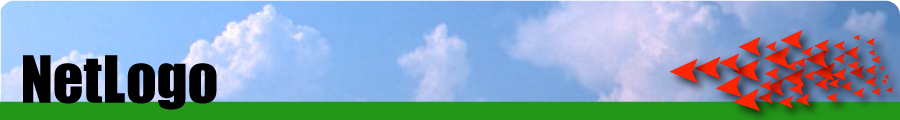
\includegraphics[width=0.7\linewidth]{figuras/netlogo-title-wide-60}
	%		\caption{}
	\label{fig:netlogo-title-wide-60}
\end{figure}	
		\vspace{-1cm}
\maketitle
}
%\setbeamertemplate{background}{\includegraphics[width=2 cm]{logo_FCEA.png}}

\begin{frame}
\frametitle{Contenido de la clase:}
\begin{itemize}
\item Redes en Economía
\item Redes como grafos
\item Notación
\item Estadísticas de redes
\item Medidas de centralidad
\item Redes de 'mundo pequeño'
\item Homofilia y segregación
\end{itemize}
\end{frame}

\begin{frame}{Introducción}
    \begin{itemize}
        \item ¿Qué son las redes? ¿Por qué estudiar redes? ¿Qué redes?
¿Qué herramientas?
\item Las redes son una forma de representar interacciones entre agentes.
\begin{itemize}
    \item En el caso de las redes sociales y económicas, estas unidades (nodos) suelen ser individuos o empresas.
\item Las conexiones entre ellos (enlaces) pueden representar una amplia gama de relaciones: amistad, relación comercial, canal de comunicación, etc
\end{itemize}
\item El estudio de las redes puede abarcar diferentes tipos de interacciones.
\begin{itemize}
    \item Redes de comunicación (Web, Internet, redes sociales).
    \item Transporte.
\item  Estructura organizativa.
\item  Comercio e intermediación.
\item  Crédito y flujos financieros.
\item Amistad o confianza.
\item Propagación de enfermedades epidémicas.
\item Difusión de productos, innovaciones e ideas.
\end{itemize}
    \end{itemize}
\end{frame}


\begin{frame}{Introducción}
\framesubtitle{COVID}
Los modelos epidemiológicos más simples ignoran la estructura de la red y las heterogeneidades entre los diferentes tipos de personas.\\
Sin embargo, los modelos estándar omiten dos ingredientes cruciales:
\begin{itemize}
 \small   \item Estructura y heterogeneidades de la red física (“teoría de grafos”): algunas personas son mucho más activas que otras y ocupan diferentes posiciones en la red de interacciones sociales (que evoluciona con el tiempo, pero no tanto como bajo una distribución uniforme).
\item Respuestas comportamentales individuales ("teoría de juegos"): en respuesta a un impacto importante como una pandemia, las personas ajustan su comportamiento "estratégicamente".
\begin{itemize}
\footnotesize    \item Cuando la enfermedad está en su apogeo, muchas personas reducirán sus niveles de actividad incluso si hay poca o ninguna intervención del gobierno. 
    \item Cuando los niveles de infección son más bajos, muchas personas aumentarán la actividad, incluso si el gobierno intenta mantener el distanciamiento social o los confinamientos.
\end{itemize}
\end{itemize}
\end{frame}


\begin{frame}{Introducción}
    \framesubtitle{El estudio de redes económicas y sociales}
La pandemia es solo un ejemplo en el que un análisis sólido depende de la comprensión tanto de la estructura de la red social como del comportamiento estratégico.
\begin{itemize}
    \item Muchas interacciones humanas están “en red” y también involucran decisiones individuales.
\item Por lo tanto, gran parte del análisis de redes se centra en las redes sociales y económicas (incluso cuando el interés principal puede estar en la comprensión de las redes físicas o de comunicación).
\begin{itemize}
    \item Por ejemplo, las estructuras de las redes sociales, como Facebook, se superponen a la Web.
\end{itemize}
\item Las redes sociales y económicas se caracterizan tanto por los patrones en los vínculos como por las interacciones y decisiones que tienen lugar entre los vínculos.
\item La mayoría de estas decisiones se toman de una manera “estratégica” y orientada a objetivos.
\end{itemize}
\end{frame}

\begin{frame}{Introducción}
\framesubtitle{Importancia de las Redes en la Economía}
\begin{itemize}
\small    \item La economía se trata de la asignación de recursos escasos: intercambio, cooperación y competencia, agregación de aprendizaje e información, adopción de tecnología, etc.
\item En realidad, gran parte de esta asignación tiene lugar en entornos en red, donde los participantes con relaciones cercanas a largo plazo interactúan en el contexto de las relaciones de otros individuos y de instituciones económicas como empresas y mercados.
\item Pero, gran parte de la economía estudia uno de los dos extremos:
\begin{enumerate}
    \item Mercados con interacciones anónimas entre un gran número de participantes.
\item  Juegos con un número reducido de jugadores.
\end{enumerate}
\begin{itemize}
    \item Ejemplo: equilibrio competitivo en un extremo, negociación y subastas en el otro.
\end{itemize}
\item ¿Podemos desarrollar nuevos conocimientos analizando sistemáticamente la red de relaciones subyacente?
    \end{itemize}
\end{frame}

\begin{frame}{Redes}
Las redes son objetos ``complicados''. Esta ``complejidad'' afecta la forma en que estudiamos las redes.
\begin{itemize}
    \item   En una red con N nodos, hay N (N -1)/2 enlaces posibles. (¿Por qué?)
\item  Cada uno de estos enlaces puede estar presente o ausente, por lo que hay $2^{N (N -1 )/2}$ redes diferentes con N nodos.
\item $\longrightarrow$hay más redes con 20 nodos que partículas elementales en el universo
\item Y la mayoría de las redes ``interesantes'' tienen más de 20 nodos. 
\end{itemize}
\end{frame}

\begin{frame}{Redes}
La gran cantidad de redes implica que nunca podemos esperar comprender completamente cada una de ellas.
\begin{itemize}
    \item En su lugar, se desarrollan marcos teóricos para identificar las propiedades clave de las redes y los procesos que se desarrollan en ellas.
\item Hasta cierto punto, estos marcos dependerán de la aplicación, pero también hay puntos en común importantes.
\item Por ejemplo, hay puntos en común, pero también diferencias importantes, en los factores que determinan la propagación de una enfermedad epidémica frente a la propagación de una nueva tecnología.
\end{itemize}
\end{frame}


\begin{frame}{Redes como grafos}
    \begin{itemize}
        \item Por lo general, representamos redes matemáticamente como grafos, que formalizan los patrones de relaciones (enlaces) entre diferentes unidades (nodos).
\item Los grafos pueden ser dirigidos o no dirigidos, según el tipo de relación que representen.
\begin{itemize}
    \item los enlaces web son dirigidos, el grafo de amigos de Facebook no está dirigido, etc.
\end{itemize}
\item Los grafos también pueden ser ponderados o no, dependiendo de si los vínculos difieren en su importancia, capacidad, probabilidad de materializarse, etc.
\begin{itemize}
    \item Ejemplo: lazos débiles vs fuertes
\end{itemize}
\item En el nivel más simple, un grafo (no ponderado) es $G =(N,E)$, donde: 
\begin{itemize}
    \item N = conjunto de n nodos en el grafo (por ejemplo, sitios web, individuos)
\item E = conjunto de aristas, nodos de enlace en el grafo
\end{itemize}
    \end{itemize}
\end{frame}

\begin{frame}{Redes como grafos}
    \framesubtitle{Notación para enlaces y grafos dirigidos /no dirigidos}
    \begin{itemize}
        \item Escribimos $i \in N$ si $i$ es un nodo de esta red, y $(i, j ) \in E$ si
existe un link desde $i$ a $j$.
\item  En un grafo no dirigido, $(i, j ) \in E$ si y sólo si $(j, i ) \in E$.
\item En un grafo dirigido, $(i, j ) \in E$ no necesariamente implica que $(j, i ) \in E$.
    \end{itemize}
\end{frame}

\begin{frame}{Notación alternativa: matriz de adyacencias}
  \begin{itemize}
      \item También podemos usar la notación $g_{ij} = 1$ si $(i, j ) \in E$ y $g_{ij} = 0$ en caso contrario.
\item Entonces la matriz $g_{ n \times n} = (g_{ij} )_{(i ,j ) \in n \times n}  $ contiene toda la información sobre quién está vinculado a quién.
\item Esta matriz se llama matriz de adyacencia del grafo.
\item Con esta información podemos hacer álgebra matricial simple en $g$ para derivar propiedades de redes, por ejemplo, determinar el número de caminos de cierta longitud entre dos nodos cualesquiera.
\item Para un grafo ponderado, podemos escribir $g_{ij} > 0$ si $(i, j ) \in E$ y $g_{ij} = 0$ en caso contrario.
\item En este caso, la magnitud de $g_{ij}$ corresponde a la intensidad del enlace.
  \end{itemize}  
\end{frame}

\begin{frame}{Un ejemplo:}
\framesubtitle{Familias renacentistas en Florencia. Fuente: Jackson (2010).}
    \begin{figure}
        \centering
        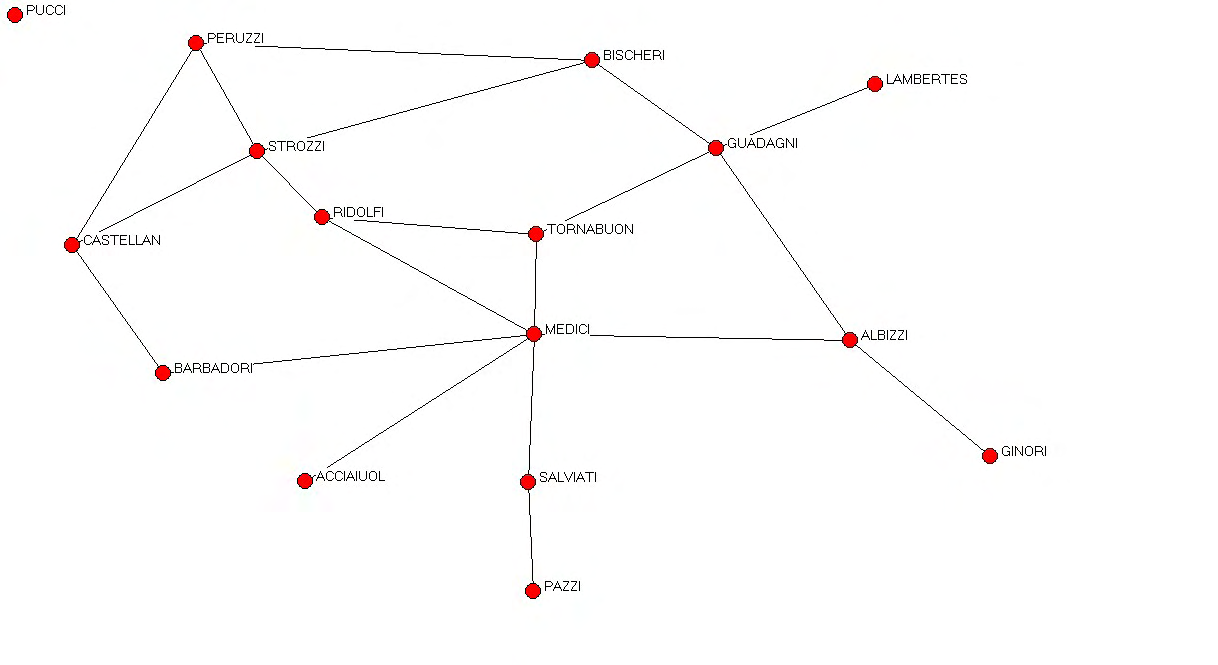
\includegraphics[width=0.7\linewidth]{figuras/medici.png}
%        \caption{\small``Florentine Marriages''. Fuente: Jackson (2010)}
        \label{fig:my_label}
    \end{figure}
Red de matrimonios en la Florencia del siglo XV.
\begin{itemize}
    \item Pensar en "matrimonio" = "alianza política", no "alma gemela".
\item ¿Cómo podemos medir el poder o "centralidad" de los Medici?    
\end{itemize}
\end{frame}

\begin{frame}{Un ejemplo:}
\framesubtitle{Familias renacentistas en Florencia (cont.)}
\begin{itemize}
    \item Los Medici están vinculados por matrimonio a más familias que nadie (6 vínculos, frente a 4 para los Strozzi y Guadagni)
\item Pero Padgett y Ansell (1994) argumentaron que el poder de los Medici no se debía solo a su número de conexiones, sino a su "centralidad" en la red social, y especialmente a su papel como "intermediarios" que unen la red.
\end{itemize}

\end{frame}

\begin{frame}{Centralidad de intermediación}
Una medida de centralidad en una red que puede capturar este rol de intermediación es la "centralidad de intermediación" o ``betweenness centrality'':
\begin{itemize}
\small 
\item Sea $P (i, j )$ el número de caminos más cortos que conectan la familia $i$ con la familia $j$.
\item Sea $P_k (i, j )$ el número de caminos más cortos que conectan estas dos familias que incluyen a la familia $k$.
\item  La \textbf{centralidad de intermediación} del nodo $k$ se define como:
\begin{equation*}
B_k \equiv \sum_{(i,j): i\neq j, k\neq i,j} \frac{P_k (i, j)/P (i, j)}{(n-1) (n-2)}
\end{equation*}
con la convención de que $P_k (i, j)/P (i, j) = 0$ si no hay un camino de $i$ a $j$.
\item Es decir, para cada par de familias $(i, j )$ calcula la fracción de los caminos más cortos que pasan por la familia $k$, y luego promedie esto sobre todos los pares $(i, j )$ sin incluir $k$.
    \end{itemize}
\end{frame}

\begin{frame}{Centralidad de intermediación}
\begin{itemize}
\small    \item Resulta que esta medida de intermediación $B_k$ es muy alta para los Médicis, 0,522.
\item El segundo $B_k$ más alto es 0,255 (la familia Guadagni).
\item Esto habría sido difícil de "observar".
\item Entonces, tal vez, los Medici estaban excepcionalmente bien posicionados para coordinar las acciones de diferentes familias, y fueron esenciales para mantener unida la red de alianzas en Florencia.
\item Sus principales rivales eran los Albizzi, mucho menos centrales.
\item En un enfrentamiento clave en septiembre de 1434, los Albizzi pidieron a otras familias que enviaran hombres armados para evitar que los Medici tomaran el gobierno, pero las otras familias no respondieron a tiempo, mientras que los Medici rápidamente obtuvieron el apoyo armado de varias familias.
\item ¿Es esta una buena medida del “poder social”? ¿Del poder político?
¿Qué aporta a nuestra comprensión? ¿Qué deja fuera?
\end{itemize}    
\end{frame}

\begin{frame}{Un ejemplo de “efectos de red”: encontrar un trabajo}
¿Cómo encuentra trabajo la gente?    
 \begin{itemize}
\small    \item Myers y Shultz (1951) \textit{The Dynamics of a Labor Market} y Rees y Shultz (1970) \textit{Workers in an Urban Labor Market} documentaron que la mayoría de los trabajadores encontraron su trabajo a través de “un contacto social”.
\item Granovetter (1973) “The Strength of Weak Ties”: la mayoría de las personas encuentran trabajo a través de conocidos, no de amigos cercanos.
\item ¿Es esto sorprendente?
\item  Sí y no. No, porque las personas tienen muchos más conocidos que amigos, sino también por la agrupación: si 1 y 2 son amigos cercanos, y 2 y 3 son amigos cercanos, entonces es muy probable que 1 y 3 se conozcan.
\item Por lo tanto, es más probable obtener referencias a un Gerente que aún no conoce a través de un conocido que un amigo cercano.
\item Esto se conoce como \textit{la fuerza de los lazos débiles}.

    \end{itemize}
\end{frame}

\begin{frame}{Clausura triádica}
    \begin{itemize}
\small        \item Veamos un ejemplo sencillo de análisis de redes, que formaliza la “fuerza de los lazos débiles” de Granovetter.
\item Representemos un grafo ponderado (no dirigido) como $G = (N,E,E')$, donde $E' \subset E$ representa "lazos fuertes".
\item $(i, j ) \in E$ significa que $i$ y $j$ son conocidos, mientras que $(i, j ) \in E'$ significa que i y j son buenos amigos.
\item La propiedad de \textbf{clausura triádica} de lazos fuertes es la siguiente:
\begin{equation*}
\text{si }(i, j) \in E'\text{ y }(j, k) \in E'\text{, entonces }(i, k ) \in E .
\end{equation*}
\item Esta propiedad se viola a menudo, por lo que podemos considerar una versión "probabilística", donde decimos que la probabilidad condicional de que $(i, k ) \in E $ (dado $(i, j) \in E'$ y $(j, k) \in E'$) es mayor que la probabilidad incondicional de $(i, k ) \in E $: es decir, 
    \end{itemize}
    \begin{equation*}
    \begin{split}
        \mathbb{P}((i, k) \in E | (i, j) \in E' \cap (j, k) \in E') > %\\
        \mathbb{P}((i, k) \in E)
        \end{split}
    \end{equation*}
\end{frame}

%%%%%%%%%%%%%%%%%
\begin{frame}{Ejemplo Conceptual: ¿Vivimos en un Mundo Pequeño?}
\begin{itemize}\small
  \item A principios del siglo XX, el poeta y escritor húngaro Frigyes Karinthy fue el primero en proponer la idea de que vivimos en un "mundo pequeño". Sugirió que dos personas entre los 1.5 mil millones de habitantes de la Tierra (de ese momento) estaban conectadas a través de un máximo de cinco conocidos.
  \item El sociólogo Stanley Milgram hizo famosa esta idea en su estudio "The Small World Problem" (1967).
  \item Milgram pidió a algunos residentes de Wichita y Omaha que enviaran una carta a una persona objetivo en Boston, pasándola primero a un conocido personal, quien haría lo mismo, y así sucesivamente hasta que se alcanzara a la persona objetivo.
  \item Esto permitió a Milgram medir cuántos "nodos intermedios" serían necesarios para vincular al remitente original con la persona objetivo.
  \item 42 de las 160 cartas supuestamente llegaron a su destinatario, con un número medio de intermediarios igual a 5.5.
\end{itemize}
\end{frame}

\begin{frame}{¿Vivimos en un Mundo Pequeño? (cont.)}
\begin{itemize}
  \item Así nació la idea de los seis grados de separación.
  \item ¿Por qué el procedimiento de Milgram podría dar resultados engañosos? (¿Una estimación demasiado baja? ¿Demasiado alta?)
  \item Existen estudios similares para otros tipos de redes.
  \item Por ejemplo, Albert, Jeong y Barabasi ("Diameter of the World Wide Web", 1999) estimaron que en 1998 se necesitaban, en promedio, 11 clics para pasar de un sitio web aleatorio a otro (en ese momento había 800 millones de sitios web).
  \item ¿Qué implican estos resultados del "mundo pequeño" sobre otros aspectos de la estructura de la red?
  \item ¿Son sorprendentes?
  \item ¿Cómo deberíamos interpretar estos resultados?
\end{itemize}
\end{frame}
\begin{frame}{Interpretando los Mundos Pequeños: Un Modelo Simple}
\begin{itemize}
  \item Supongamos que cada nodo tiene $\lambda$ vecinos (por ejemplo, cada sitio web tiene enlaces a $\lambda$ otros sitios web).
 % \item Cada uno de mis $\lambda$ vecinos tendrá a su vez $\lambda$ vecinos.
  \item Supongamos, de manera poco realista, que mis vecinos no tienen vecinos en común (esto no puede ser del todo correcto, porque mis vecinos tienen al menos un vecino en común, que soy yo, pero a veces es una buena aproximación).
  \item Entonces, en dos pasos, puedo llegar a $\lambda^{2}$ otros nodos.
  \item Repitiendo el mismo razonamiento (y manteniendo la misma suposición simplificadora), en $d$ pasos puedo llegar a $\lambda^{d}$ otros nodos.
  \item Ahora imagina que esta red tiene $n \approx \lambda^{d}$ nodos.
  \item Esto implica que el "grado de separación" (la distancia media entre dos nodos) es aproximadamente
\end{itemize}

$$
d=\frac{\ln n}{\ln \lambda}
$$

\end{frame}

\begin{frame}{Interpretando los Mundos Pequeños (cont.)}
\begin{itemize}
  \item Supongamos que tomamos la fórmula $d=\ln n / \ln \lambda$ como una primera aproximación plausible para el "grado de separación".
  \item Supongamos que, como en la época de Karinthy, la población mundial es de aproximadamente 2 mil millones. ¿Cuántos amigos necesitaría tener cada persona para que el grado de separación sea igual a 5?
  \item Resolviendo nuestra fórmula para $\lambda$, obtenemos
\end{itemize}

$$
\lambda=\exp \left(\frac{\ln n}{d}\right)
$$

Sustituyendo $n=2$ mil millones y $d=5$ obtenemos

$$
\lambda=\exp \left(\frac{\ln 2,000,000,000}{5}\right) \approx 72
$$

\begin{itemize}
  \item Así que la "separación de cinco grados" de Karinthy no era una suposición descabellada (o al menos coincide con nuestro modelo simple).
\end{itemize}
    
\end{frame}


\begin{frame}{Interpretando los Mundos Pequeños (cont.)}
\begin{itemize}
  \item Cuando Milgram escribió a mediados de la década de 1960, la población mundial era de aproximadamente 3.5 mil millones. Para que el grado de separación sea igual a 6, el número de amigos que necesitaría tener cada persona sería aproximadamente
\end{itemize}

$$
\exp \left(\frac{\ln 3,500,000,000}{6}\right) \approx 39
$$

\begin{itemize}
  \item No es un número muy diferente.
\end{itemize}
\end{frame}

\begin{frame}{Interpretando los Mundos Pequeños (cont.)}
\begin{itemize}
  \item La suposición simplificadora de que mis vecinos no son vecinos entre sí se llama aproximación de proceso de ramificación.\\
  Imagina la red como un "árbol", cuando en realidad no lo es.
  \item A veces esto es muy útil; otras veces puede ser engañoso.
  \item Esta suposición descarta triángulos o ciclos (y, en general, la agrupación, una medida de la densidad de triángulos), que son muy comunes en redes sociales, enlaces web y otras redes.
  \item Sin embargo, curiosamente, en los grafos aleatorios de Erdos-Renyi, donde los enlaces se forman de manera uniforme al azar, veremos que la distancia promedio puede aproximarse para grandes $n$ mediante $d=\ln n / \ln \lambda$ (donde $\lambda$ es el grado esperado de un nodo).
  \item Esto se debe a que los ciclos son relativamente raros en tales grafos.
\end{itemize}
    
\end{frame}

\begin{frame}{Interpretando los Mundos Pequeños (cont.)}
\begin{itemize}
  \item La falta de ciclos es una forma en la que los grafos aleatorios de Erdos-Renyi, aunque matemáticamente convenientes, no son buenas aproximaciones a las redes sociales.
  \item En realidad, el camino más corto entre personas remotas generalmente pasa por "conectores" especiales, como su amigo más popular, un primo en otra ciudad o un representante político.
  \item Los modelos de redes de mundo pequeño modifican el modelo de grafo aleatorio de Erdos-Renyi para intentar capturar este tipo de patrón (aunque no siempre perfectamente).
\end{itemize}
    
\end{frame}



\begin{frame}{Tipos de redes en el mundo real}
    \begin{itemize}
        \item Una red es un conjunto de unidades (nodos o vértices) conectadas por relaciones (enlaces o aristas).
\item Tipos de redes:
\begin{itemize}
    \item Redes sociales y económicas: los nodos son personas o grupos de personas.
    \begin{itemize}
    \item Redes de amistad, relaciones comerciales entre empresas, matrimonios mixtos entre familias, relaciones laborales en el mercado de trabajo
    \end{itemize}
\item Redes de información: los nodos son “objetos de información”
\begin{itemize}
    \item Enlaces web, red de citas entre artículos académicos, redes semánticas/de clasificación (taxonomías)
\end{itemize}
\item Redes tecnológicas
\begin{itemize}
    \item Redes de infraestructura como internet, red eléctrica, redes de transporte
\item  Redes temporales como redes de sensores, vehículos autónomos
\end{itemize}
\item Redes biológicas
\begin{itemize}
    \item Red alimentaria, red de interacción de proteínas, red neuronal, red de vías metabólicas
\end{itemize}
\end{itemize} 
    \end{itemize}
\end{frame}

\begin{frame}[allowframebreaks]
\frametitle{Redes}
Estudio histórico de las redes:
    \begin{itemize}
        \item Teoría matemática de grafos: parte central de la matemática discreta
\begin{itemize}
    \item Comenzó con la solución de Euler de 1735 al problema del puente de Königsberg.
    \begin{figure}
        \centering
        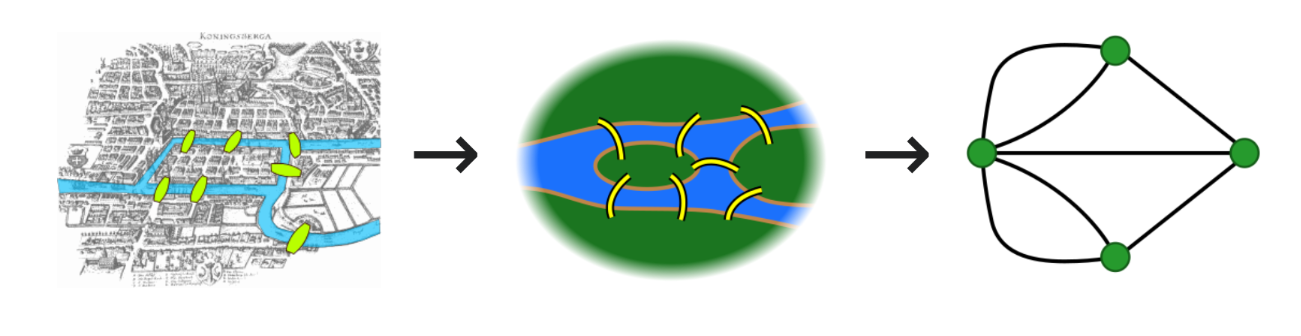
\includegraphics[width=\linewidth]{Captura desde 2024-10-01 15-49-39.png}
  %      \caption{Caption}
        \label{fig:enter-label}
    \end{figure}
\end{itemize}
\item Análisis de redes sociales en ciencias sociales.
\begin{itemize}
    \item Los estudios típicos involucraron la circulación de cuestionarios, lo que llevó a redes relativamente pequeñas; también poco enfoque en el comportamiento individual.
\end{itemize}
    \end{itemize}

Los últimos años han sido testigos de un cambio sustancial en la investigación de redes.
\begin{itemize}
    \item Desde el análisis de pequeños grafos individuales (<100 nodos) hasta las propiedades estadísticas de redes a gran escala (millones/billones de nodos).
        \item Motivado por la disponibilidad de computadoras y datos informáticos.
\end{itemize} 
\end{frame}


\begin{frame}{Grafos}
    \begin{itemize}
 \small       \item Un \textbf{grafo} consta de un conjunto de nodos $N = \{1, . . . , n \}$ y una matriz $n \times n$ $g = [g_{ij}]_{i,j \in N}$ llamada matriz de adyacencia, donde $g_{ij} \in {0,1}$ denota la ausencia/presencia de una arista desde el nodo $i$ hasta el nodo $j$.
\item En un grafo ponderado, el peso de la arista $g_{ij} > 0$ puede tomar valores no binarios, que representan la intensidad de la interacción.
\item En un grafo no dirigido, $g_{ij} = g_{ji} \text{ } \forall  i, j \in N $ ($g$ es simétrica).
\begin{itemize}
    \item por ejemplo amigos de Facebook
\end{itemize} 
\item En un grafo dirigido (dígrafo), $g_{ij}$ y $g_{ji}$ pueden diferir.
\begin{itemize}
    \item por ejemplo enlaces web
\end{itemize} 
\item Ejemplos: dibujar los grafos correspondientes a matrices de adyacencia:
    \end{itemize}
    \begin{columns}
    \centering
\begin{column}{0.5\textwidth}
\centering %(1)
\begin{equation}
  \begin{bmatrix}
0 & 1 & 0\\
0 & 0 & 1 \\
1 & 0 & 0
\end{bmatrix}  
\end{equation}
\end{column}
\begin{column}{0.5\textwidth} \centering %(2)
\begin{equation}
     \begin{bmatrix}
0 & 0 & 1\\
1 & 0 & 0 \\
1 & 1 & 0
\end{bmatrix}
\end{equation}

\end{column}
\end{columns}
\end{frame}

\begin{frame}{Grafos}
 \begin{itemize}
     \item De manera equivalente, se puede representar un grafo por $(N, E )$, donde $E \subseteq N \times N$ es el conjunto de aristas.
\item Para grafos dirigidos, $E$ es el conjunto de aristas “dirigidas”, $(i, j ) \in E $.
\item Para grafos no dirigidos, $E$ es el conjunto de aristas “no dirigidas”,  $(i, j ) \in E $ .
\begin{itemize}
    \item Ejemplo 1: $Ed = \{(1, 2) , (2, 3) , (3, 1)\}$
    \item Ejemplo 2: podría escribirse como $Eu = \{\{1,2\}, \{1,3\}, \{2,3\}\}$ o $Ed = \{(1,2), (2,1), (2,3), (3,2), (3,1), (1,3)\}$
\end{itemize}
\item A veces denotamos $g_{ij} = 1$ con la notación $(i, j ) \in g$ , o ${i, j } \in g $, o incluso $ij \in g $.
 \end{itemize}   
\end{frame}

\begin{frame}{Grafos}
    \framesubtitle{Conectividad y componentes}
 \begin{itemize}
     \item Un grafo no dirigido es \textbf{conexo} si por cada dos nodos existe un camino entre ellos.
\item Un grafo (N',E') es un subgrafo de (N,E) si $N' \subset N, E' \subset E$, y ${i, j } \in E'$ implica $i, j \in N'$ . (Cada enlace debe tener extremos).
\item Un componente de un grafo es un subgrafo conexo máximo.
\item  Es decir, un subgrafo conexo que no está contenido en ningún subgrafo conexo mayor.
\item Una arista {i, j } es un \textbf{puente} si al eliminarla aumenta el número de componentes.
 \end{itemize}   
 Nota: la matriz de adyacencia de un grafo con más de un componente se puede escribir en forma de bloques diagonales: es decir, los 1's están confinados a bloques cuadrados a lo largo de la diagonal, con todos los demás elementos iguales a 0.
\end{frame}

\begin{frame}{Grafos}
    \framesubtitle{Conectividad y componentes en grafos dirigidos}

Un grafo dirigido se encuentra:    
    \begin{itemize}
        \item \textbf{conectado} si el grafo no dirigido subyacente está conectado (es decir, ignorando las direcciones de los bordes).
        \item \textbf{fuertemente conectado} si cada nodo puede llegar a todos los demás nodos por un "camino dirigido".
            \end{itemize}

Un componente fuertemente conectado es un subgrafo máximo fuertemente conectado. Eso es,
\begin{enumerate}
\item  Cada nodo en el subgrafo puede llegar a cualquier otro nodo en el subgrafo por un camino dirigido contenido en el subgrafo.
\item El subgrafo no esta contenido en ningun subgrafo mayor con esta propiedad.
\end{enumerate}
\end{frame}

\begin{frame}{Grafos}
\framesubtitle{Algunos grafos especiales}
    \begin{itemize}
 \small       \item Una \textbf{clique} (o \textbf{red completa}) es un grafo donde todos los nodos están vinculados entre sí.
\item Un \textbf{árbol} es un grafo conectado (no dirigido) sin ciclos.
\begin{itemize}
\item Un grafo \textbf{conexo} es un árbol si y solo si tiene $n - 1$ aristas.
\item En un árbol, hay un camino único entre dos nodos cualesquiera.
\end{itemize}
\item Un \textbf{bosque} es un grafo en el que cada componente es un árbol.
\item Una \textbf{estrella} es un árbol en el que un nodo (el centro) está vinculado a todos los demás nodos.
\item Un \textbf{anillo} (o círculo, o ciclo) es un grafo conectado donde cada nodo está vinculado a otros dos.
\item Un \textbf{grafo bipartito} es aquel que se puede dividir en dos conjuntos de modo que todos los enlaces conecten nodos en conjuntos "opuestos".
\begin{itemize}
    \item Compradores y vendedores, empresas y trabajadores, estudiantes y escuelas, hombres y mujeres
\end{itemize}
    \end{itemize}
\end{frame}

\begin{frame}{Estadísticas de redes}
    \begin{itemize}
        \item Las redes pequeñas se pueden visualizar directamente, pero las redes más grandes son más difíciles de visualizar y describir.
\item Por lo tanto, es útil definir varias estadísticas de resumen para describir y comparar redes (aquí centrándonos principalmente en grafos no dirigidos):
\begin{itemize}
\item Distribución de grado (¿qué tan densa?)
\item Diámetro y longitud de trayectoria promedio (¿qué tan estrechamente conectados?)
\item Agrupación (¿los amigos de los amigos son amigos?)
\item Centralidad (¿qué nodos son centrales o importantes?)
\item Homofilia (¿es más probable que los nodos del mismo "tipo" estén vinculados?)
\end{itemize}
    \end{itemize}
\end{frame}

\begin{frame}{Vecindad y grado}
\begin{itemize}
\item La vecindad, $N_i$, del nodo $i$ es el conjunto de nodos a los que está vinculado: $N_i = \{j : g_{ij} = 1\}.$
\item Para grafos no dirigidos, el grado, $d_i$, del nodo $i$ es su número de vecinos, o de manera equivalente, la cardinalidad de su vecindad: $d_i = \sum_j g_{ij} = \sum_j g_{ji} = \#N_i$.
\item Para grafos dirigidos,
\begin{itemize}
 \item El grado de salida (\textbf{out-degree}) del nodo $i$ es $\sum_j g_{ij}$ .
\item  El grado de entrada (\textbf{in-degree}) del nodo $i$ es $\sum_j g_{ji}$.
\end{itemize}
\item También figuran a veces los términos “out-neighbor” y “in-neighbor”.
\item En las aplicaciones, si un enlace de $i$ a $j$ significa que $i$ “influye” en $j$, los nodos con alto out-degree son “influyentes”.
\item Si un enlace significa que $i$ "escucha" o "respalda" $j$ (por ejemplo, un hipervínculo a $j$), los nodos con alto grado de entrada son influyentes.
    \end{itemize}
\end{frame}


\begin{frame}{Grado medio, densidad, dispersión}
    \begin{itemize}
        \item El grado promedio, $\bar{d}$ de una red no dirigida, es:
        \begin{equation*}
            \bar{d}=\frac{1}{n}\sum_i d_i
        \end{equation*}
        
\item Considerar que si la red tiene un total de $m$ aristas, entonces tenemos
$\sum_i d_i= 2m$.

Por tanto, $\bar{d} = 2m/n$.
\item La densidad, $\rho$, de una red no dirigida es la fracción de todos los posibles enlaces que realmente existen, dados por
        \begin{equation*}
            \rho=\frac{m}{n(n-1)2}=\frac{\bar{d}}{n-1}
        \end{equation*}

\item Para redes grandes, a menudo se aproxima como $\frac{\bar{d}}{n}$.
\item Una red es \textbf{dispersa} si $\rho$ es pequeño.
\item Cuando se habla de redes grandes, a menudo se entiende que esto significa
que $\rho \longrightarrow 0$ cuando $n \longrightarrow \infty$.
    \end{itemize}
\end{frame}

\begin{frame}{Distribución de grado}
    \begin{itemize}
        \item La distribución de grados, $P (d)$, de una red describe la proporción de nodos que tienen diferentes grados $d$.
\item Para un grafo dado, $P (.)$ es un histograma: es decir, $P (d)$ es la fracción de nodos con grado $d$.
\item Para un modelo de grafo aleatorio, $P (.)$ es una distribución de probabilidad: es decir, $P (d)$ es la probabilidad de que un nodo tenga grado $d$.
\item Un grafo es $d-regular$ si todos los nodos tienen el mismo grado $d$.
\item Dos tipos de $P (d)$ para modelos de grafos aleatorios:
\begin{itemize}
    \item con decaimiento exponencial
    \item siguiendo una \textit{power-law}
    \begin{itemize}
        \item También conocida como distribución libre de escala: una distribución que no cambia (dentro de un factor multiplicativo) bajo un cambio de escala de la variable.
\item Aparecen lineales en un gráfico log-log.
    \end{itemize}
\end{itemize}
    \end{itemize}
\end{frame}

\begin{frame}{Diámetro y camino promedio}
    Sea $\ell(i, j)$ la distancia (longitud del camino más corto) entre los nodos $i$ y $j$.

El \textbf{diámetro} de una red conexa se define como la mayor distancia entre cualquier par de nodos:

$$
\text{diámetro} = \max_{i, j} \ell(i, j)
$$

La \textbf{longitud promedio del camino} es la distancia promedio entre cualquier par de nodos:

$$
\text{longitud promedio del camino} = \frac{\sum_{i \neq j} \ell(i, j)}{n(n-1)}
$$

La longitud promedio del camino está acotada superiormente por el diámetro. En algunos casos, es mucho más corta que el diámetro.

Si la red no está conectada, se suele calcular el diámetro y la longitud promedio del camino en el componente conexo más grande.
\end{frame}


\begin{frame}{Clustering}
    \begin{itemize}
        \item Mide hasta qué punto mis amigos son amigos entre sí.
\item La medida más simple es el coeficiente de agrupamiento global $Cl(g)$, dado por 
\begin{equation*}
Cl (g ) =\frac{ 3 \times \text{ número de triángulos en la red}}{\text{número de “triángulos potenciales”}}
\end{equation*}
 donde un “triángulo potencial” es un triple de nodos distintos $(i, j, k )$ tal que $g_{ij} = g_{ik} = 1$.

     \item Tener en cuenta que $0 \leq Cl (g ) \leq 1$.
\item  También conocida como transitividad de la red: mide el grado en que un amigo de mi amigo también es mi amigo.
    \end{itemize}
\end{frame}


\begin{frame}{Clustering}
\begin{itemize}
 \small   \item Una medida diferente de la agrupación se basa en medir primero la "agrupación individual" para cada nodo $i$ y luego promediar los nodos.
\item El \textbf{agrupamiento individual para el nodo $i$} es el número de triángulos que involucran $i$, 

\begin{equation*}
Cl_i (g )=\frac{ \text{número de triángulos centrados en i}}{\text{número de triángulos potenciales centrados en i}}
\end{equation*}

\item El \textbf{coeficiente de agrupamiento promedio} es $Cl^{Avg} (g ) = \frac{1}{n} \sum_i Cl_i (g ) $.
\item Considere la red de "molino de viento" no dirigida, donde todos están conectados al centro y a otro nodo.
\begin{itemize}
    \item El agrupamiento promedio es cercano a 1, porque $Cl_i (g ) = 1$ para todos excepto el centro.
\item  El agrupamiento general es cercano a 0, porque la gran mayoría de los triángulos potenciales consisten en el centro y dos individuos que no están vinculados.
\end{itemize} 
\end{itemize}
\end{frame}

\begin{frame}{Medidas de centralidad}
    \begin{itemize}
        \item Hay varias medidas que capturan alguna noción de la "centralidad" o "importancia" de un nodo en una red.
\item Diferentes medidas capturan diferentes nociones de centralidad, que son importantes para responder diferentes preguntas.
\item Grado de centralidad: Simplemente grado dividido por (n-1).
\item Centralidad de cercanía/decaimiento: “En promedio”, ¿qué tan cerca está el nodo de otros nodos?
\item Una medida simple: distancia media inversa
\item Una medida más rica: centralidad de decaimiento, el cual depende del parámetro de decaimiento 
$\delta \in (0, 1)$.
\item Centralidad de intermediación: ¿Qué tan importante es el nodo para conectar otros nodos?
    \end{itemize}
\end{frame}

\begin{frame}{Medidas de centralidad basadas en vectores propios}
 \small Una clase más sutil y muy importante de medidas de centralidad se basa en la idea autorreferencial de que un nodo es importante si está conectado a otros nodos importantes.   
    \begin{itemize}
\small        \item Estas medidas no se pueden calcular por separado para cada nodo; en cambio, calculamos la medida para todos los nodos simultáneamente a través de un sistema de ecuaciones.
\item Estas medidas se denominan colectivamente medidas de centralidad basadas en vectores propios (porque el cálculo implica vectores propios). Tienen muchas aplicaciones, incluida la comprensión:
\begin{itemize}
\item Cómo clasifica Google las páginas web (PageRank).
\item Qué agentes en una red social son influyentes en la formación de la opinión de consenso a largo plazo del grupo (aprendizaje DeGroot).
\item Qué empresas en una red de producción son las más importantes desde el punto de vista sistémico (análisis insumo-producto de Leontieff).
\item . . . y más.
\end{itemize}
    \end{itemize}
\end{frame}


\begin{frame}{Homofilia y segregación}
\begin{itemize}
    \item Finalmente, otro tipo de estadística de red es útil cuando los nodos son de diferentes tipos o pertenecen a diferentes grupos.
\item Individuos de diferente género, raza, edad, afiliación política, religión, educación, etc.
\item  Blogs liberales vs. conservadores (u otros medios)
\item En estos entornos, una pregunta clave es el grado de homofilia: la medida en que es más probable que los nodos del mismo tipo estén conectados.
\begin{itemize}
\item  “La similitud engendra amistad” – Platón
\item  “La gente ama a los que son como ellos mismos” – Aristóteles
\item  “Las aves del mismo plumaje vuelan juntas” – Proverbio
\end{itemize}
\end{itemize}    
\end{frame}

\begin{frame}[allowframebreaks]
\frametitle{Midiendo la homofilia}
\begin{itemize}
    \item Hay diferentes formas de medir la homofilia, pero la más simple es observar la fracción de enlaces que realmente existen entre individuos de diferentes tipos, en relación con lo que se esperaría si los enlaces se formaran uniformemente al azar.
    \item Supongamos que la fracción $p_{1}$ de la población es del grupo 1 y la fracción $p_{2}$ de la población es del grupo 2. (Puede haber también otros tipos.)
    \item Si los enlaces estuvieran distribuidos aleatoriamente, la fracción $p_{1}^{2}$ de los enlaces conectaría dos nodos del grupo 1, y la fracción $2 p_{1} p_{2}$ conectaría un nodo del grupo 1 y un nodo del grupo 2.
    \item Si fijamos un enlace y asignamos aleatoriamente el nodo en cada extremo al tipo 1 o al tipo 2, obtenemos dos del tipo 1 con probabilidad $p_{1}^{2}$ y uno de cada tipo con probabilidad $2 p_{1} p_{2}$.
    \item Por lo tanto, si la fracción de enlaces dentro del grupo 1 está significativamente por encima de $p_{1}^{2}$, esto es evidencia de homofilia (o "emparejamiento asortativo") dentro del grupo 1.
    \item Si la fracción de enlaces entre el grupo 1 y el grupo 2 está significativamente por debajo de $2 p_{1} p_{2}$, esto es evidencia de homofilia/asortatividad dentro de los grupos, o segregación/disasortatividad entre ellos.
\end{itemize}
\end{frame}

\begin{frame}{Introduciendo la Centralidad de Autovector}
La medida más simple es la centralidad de autovector: un vector no nulo $C=\left(C_{i}\right)_{i \in N}$ tal que, para algún escalar $\lambda>0$, tenemos
$$
\lambda C_{i}=\sum_{j \neq i} g_{j i} C_{j} \text { para todo } i \in N
$$
Es decir, la centralidad de cada nodo $i$ es proporcional a la suma ponderada de la centralidad de sus vecinos.
\begin{itemize}
\item Nótese que en esta definición tenemos $g_{j i}$ en lugar de $g_{i j}$.
\item Esto no importa para grafos no dirigidos, pero para grafos dirigidos indica que la centralidad de un nodo se deriva de la centralidad de los nodos que apuntan hacia él.
\item Interpretación: cuando nodos "importantes" o "prestigiosos" apuntan hacia ti, esto te hace importante/prestigioso.
\item Las ecuaciones siguen siendo válidas si multiplicamos $C$ por un escalar. Típicamente normalizamos para que $\sum_{i \in N} C_{i}=1$.
\end{itemize}
\end{frame}

\begin{frame}{Centralidad de Autovector (cont.)}
    La centralidad de autovector $\left(C_{i}\right)_{i \in N}$ se define por:
$$
\lambda C_{i}=\sum_{j \neq i} g_{j i} C_{j} \quad \text { para todo } i \in N
$$
No es inmediatamente obvio si podemos encontrar tal vector $C$: es decir, si tal medida existe o es única.
\begin{itemize}
\item Pero, $n$ ecuaciones lineales con $n$ incógnitas...
\end{itemize}
\end{frame}
    
\begin{frame}[allowframebreaks]
\frametitle{¿Cuándo está bien definida la Centralidad de Autovector?}
Para redes fuertemente conectadas, resulta que la centralidad de autovector siempre está bien definida.
\begin{itemize}
\item Recordemos que una red dirigida está fuertemente conectada si existe un camino dirigido entre cualquier par de nodos.
\item En particular, toda red no dirigida conexa está fuertemente conectada.
\item En general, la red está fuertemente conectada si y solo si para cada par de nodos $i, j$, existe un número $\ell$ tal que $\left(g^{\ell}\right)_{i j}>0$.
\item Las matrices $g$ con esta propiedad se llaman irreducibles.
\item Es decir, una red está fuertemente conectada si y solo si su matriz de adyacencia es irreducible.
\end{itemize}
\end{frame}

\begin{frame}{¿Cuándo está bien definida la Centralidad de Autovector? (cont.)}
 En forma matricial, la ecuación para los $C_{i}$ es
$$
\lambda C=g^{T} C
$$
donde $\lambda$ es un escalar, $C$ es un vector $n \times 1$, y $g^{T}$ es la transpuesta de la matriz de adyacencia $n \times n$ (transpuesta porque, para grafos dirigidos, nos importan los nodos que te enlazan, no los nodos a los que enlazas).
\begin{itemize}
\item Es decir, $C$ es un autovector de $g^{T}$, con $\lambda$ el autovalor correspondiente.
\item El teorema de Perron-Frobenius del álgebra lineal dice que, para toda matriz no negativa irreducible, su mayor autovalor es positivo, y todas las componentes del autovector correspondiente también son positivas.
\end{itemize}
\end{frame}
\begin{frame}{¿Cuándo está bien definida la Centralidad de Autovector? (cont.)}
\begin{itemize}
\item Así, si tomamos $\lambda$ como el mayor autovalor de $g^{T}$, el autovector correspondiente $C$ es no negativo.
\item Por lo tanto, para cualquier red fuertemente conectada, el vector de centralidad de autovector $C$ está bien definido.
\end{itemize}
\end{frame}

\begin{frame}{Interpretación como Proporciones Poblacionales a Largo Plazo}\small
Una interpretación útil de la centralidad de autovector como el resultado a largo plazo de un proceso de reproducción (que también explica por qué siempre está bien definida para redes fuertemente conectadas):
\begin{itemize}
\item Supongamos que un "virus" comienza en un nodo del grafo.
\item En cada período, cada virus envía una copia de sí mismo a lo largo de cada enlace desde el nodo donde se encuentra. Luego muere.
\item (Así que hay 1 virus en el período 1, $N_{i}$ virus en el período 2, $\sum_{j \in N_{i}} N_{j}$ virus en el período 3, etc.)
\item Dejando que este proceso se ejecute para siempre, el virus nunca se extingue (porque la red está fuertemente conectada), y podemos calcular la fracción a largo plazo de virus ubicados en cada nodo.
\item La fracción a largo plazo de virus ubicados en el nodo $i$ es igual a $C_{i}$.\
(¿Por qué? Porque la fracción a largo plazo de virus ubicados en el nodo $i$ es proporcional a la fracción a largo plazo de virus ubicados en los nodos que enlazan al nodo $i$. Esta es la relación que define la centralidad de autovector.)
\end{itemize}
\end{frame}
\setbeamertemplate{blocks}[rounded]%[shadow]
\setbeamercolor{block body}{bg=structure!10}
\setbeamercolor{block title}{bg=structure!20}

\begin{frame}{Teorema de Perron-Frobenius}
\begin{block}{Teorema:}
    Para toda matriz no negativa irreducible $A$, su mayor autovalor $r_{1}$ es un número real positivo, y las componentes del autovector correspondiente $v_{1}$ también son todas positivas.
\end{block}
El teorema dice más, pero esto es lo que necesitamos.\
La demostración está fuera de nuestro alcance, pero podemos dar un argumento informal informativo.
\end{frame}
\begin{frame}[allowframebreaks]
\frametitle{Intuición para el Teorema de Perron-Frobenius}
\begin{itemize}
\item Fijemos cualquier vector no negativo $x(0) \in \mathbb{R}^{n}$. Supongamos que podemos escribirlo como una combinación lineal de los autovectores $v_{i}$ de $A$:
\end{itemize}
$$
x(0)=\sum_{i} c_{i} v_{i}
$$
\begin{itemize}
\item Consideremos multiplicar repetidamente $x(0)$ por $A$. (Multiplicación matricial = copiar virus.) Después de $t$ pasos, obtenemos el vector
\end{itemize}
$$
x(t)=A^{t} x(0)=A^{t} \sum_{i} c_{i} v_{i}=\sum_{i} c_{i} r_{i}^{t} v_{i}=r_{1}^{t} \sum_{i} c_{i}\left(\frac{r_{i}}{r_{1}}\right)^{t} v_{i}
$$
\begin{itemize}
\item Como $r_{1}$ es el mayor autovalor, $\left(\frac{r_{i}}{r_{1}}\right)^{t} \rightarrow 0$ cuando $t \rightarrow \infty$, para todo $i \neq 1$. Por lo tanto, $x(t) / r_{1}^{t} \rightarrow c_{1} v_{1}$. Es decir, el vector límite $x(\infty)$ es proporcional al mayor autovector.
\item Como $x(0)$ era no negativo y $A$ es no negativa, cada $x(t)$ también es no negativo. Por lo tanto, $r_{1}$ debe ser positivo (de lo contrario, oscilaría), y cada componente de $v_{1}$ también debe ser positiva.
\end{itemize}
\end{frame}

\begin{frame}{Otras Perspectivas de este Argumento}
Al igual que con los virus, el vector límite $x(\infty)$ es proporcional al mayor autovector. Este vector define la centralidad de autovector.
También podríamos preguntarnos qué tan rápido ocurre esta convergencia.
\begin{itemize}
\item Esto está determinado por qué tan rápido $\left(\frac{r_{2}}{r_{1}}\right)^{t}$ se acerca a 0 cuando $t \rightarrow \infty$ (ya que $\left(\frac{r_{i}}{r_{1}}\right)^{t}$ se acerca a 0 más rápido que esto para cada $i \geq 3$).
\item Una brecha mayor entre el primer y segundo autovalor $\Longrightarrow$ convergencia más rápida.
\end{itemize}
    
\end{frame}
\end{document}
